\documentclass{standalone}
\usepackage{ tikz }
\usepackage{ xparse }
\usepackage{ stmaryrd }
\input{macros/all}

\begin{document}
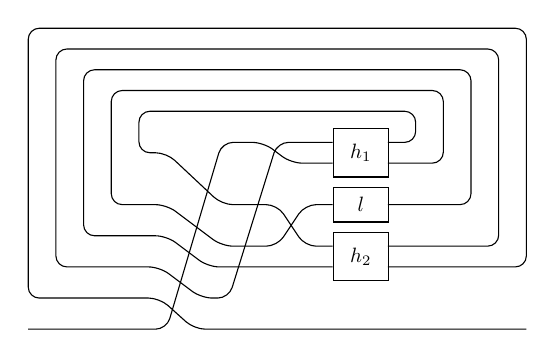
\begin{tikzpicture}[yscale=-1,x=1em,y=1.5em]

    \draw[rounded corners] (-5,4.25) -- (0, 4.25) -- (2,-0.25) -- (3.5, -0.25) -- (4.5, 0.25) -- (6,0.25);
    \draw[rounded corners] (8, 2.75) -- (13,2.75) -- (13, -3.0) -- (-5,-3) -- (-5, 3.5) -- (-0.25,3.5) -- (1, 4.25) -- (13,4.25);
    \draw[rounded corners] (8, 2.25) -- (12, 2.25) -- (12,-2.5) -- (-4,-2.5) -- (-4,2.75) -- (-0.25,2.75) -- (1.25,3.5) -- (2.25, 3.5) -- (4,-0.25) -- (6,-0.25);
    \draw[rounded corners] (8, 1.25) -- (11,1.25) -- (11,-2) -- (-3,-2) -- (-3,2) -- (0,2) -- (1.5,2.75) -- (6,2.75);
    \draw[rounded corners] (8, 0.25) -- (10,0.25) -- (10,-1.5) -- (-2,-1.5) -- (-2,1.25) -- (0,1.25) -- (2,2.25) -- (4,2.25) -- (5,1.25) -- (6,1.25);
    \draw[rounded corners] (8,-0.25) -- (9,-0.25) -- (9,-1) -- (-1,-1) -- (-1,0) -- (0,0) -- (2,1.25) -- (4,1.25) -- (5,2.25) -- (6,2.25);

    \node[draw,minimum height=1.75em,minimum width=2em,anchor=west] at (6,0) {\scalebox{0.75}{$h_1$}};
    \node[draw,minimum height=1.25em,minimum width=2em,anchor=west] at (6,1.25) {\scalebox{0.75}{$l$}};
    \node[draw,minimum height=1.75em,minimum width=2em,anchor=west] at (6,2.5) {\scalebox{0.75}{$h_2$}};

\end{tikzpicture}
\end{document}
